\documentclass[tikz,border=12pt]{standalone}
% Match the sans-serif font stack used by the Minimal Mistakes site theme.
% TeX Gyre Heros is the TeX-compatible Helvetica implementation.
\usepackage[T1]{fontenc}
\usepackage{tgheros}
\renewcommand{\familydefault}{\sfdefault}

\usetikzlibrary{arrows.meta,positioning}
\definecolor{pink}{HTML}{F72585}\definecolor{blue}{HTML}{4DABF7}\definecolor{green}{HTML}{51CF66}\definecolor{ink}{HTML}{E9ECEF}\definecolor{panel}{HTML}{211C1D}
\begin{document}
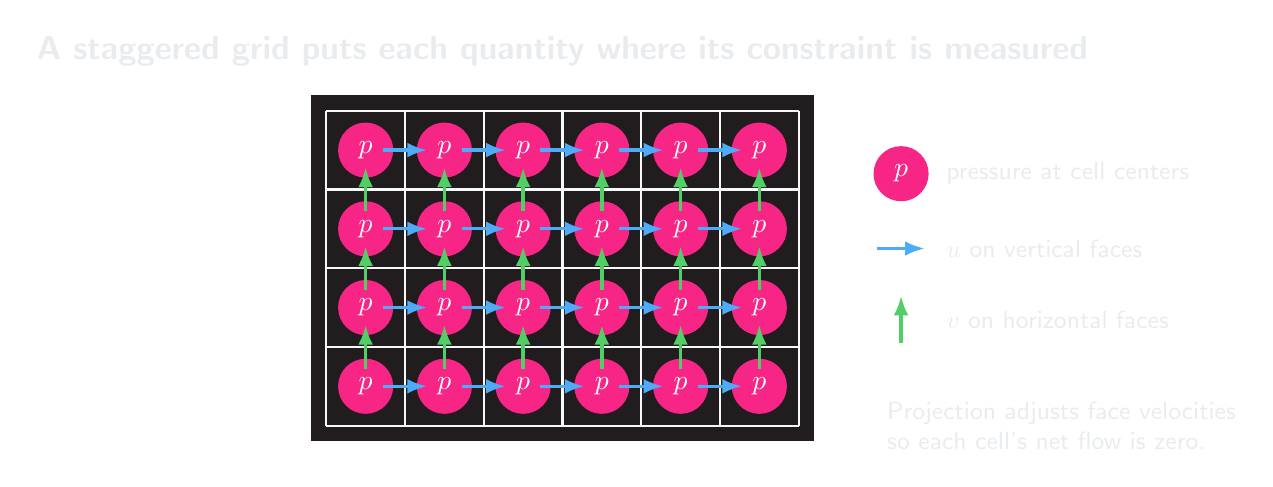
\begin{tikzpicture}[text=ink,pressure/.style={circle,fill=pink,text=white,minimum size=7mm,font=\bfseries},velocity/.style={-{Latex[length=2.5mm]},very thick,blue},grid/.style={ink!35,line width=.8pt}]
 \fill[panel] (-.2,-.2) rectangle (6.2,4.2);
 \foreach \x in {0,...,6}{\draw[grid] (\x,0)--(\x,4);}
 \foreach \y in {0,...,4}{\draw[grid] (0,\y)--(6,\y);}
 \foreach \x in {.5,1.5,...,5.5}{\foreach \y in {.5,1.5,...,3.5}{\node[pressure] at (\x,\y) {$p$};}}
 \foreach \x in {1,...,5}{\foreach \y in {.5,1.5,...,3.5}{\draw[velocity] (\x-.28,\y)--(\x+.28,\y);}}
 \foreach \x in {.5,1.5,...,5.5}{\foreach \y in {1,...,3}{\draw[velocity,green] (\x,\y-.28)--(\x,\y+.28);}}
 \node[font=\bfseries\large,text=ink] at (3,4.75) {A staggered grid puts each quantity where its constraint is measured};
 \node[pressure] (pk) at (7.3,3.2) {$p$}; \node[anchor=west,font=\small,text=ink] at (7.75,3.2) {pressure at cell centers};
 \draw[velocity] (7,2.25)--(7.6,2.25); \node[anchor=west,font=\small,text=ink] at (7.75,2.25) {$u$ on vertical faces};
 \draw[velocity,green] (7.3,1.05)--(7.3,1.65); \node[anchor=west,font=\small,text=ink] at (7.75,1.35) {$v$ on horizontal faces};
 \node[anchor=west,align=left,font=\small,text=ink] at (7,0)
  {Projection adjusts face velocities\\so each cell's net flow is zero.};
\end{tikzpicture}
\end{document}
